\subsection{The \moc{DEVINI:} module}\label{sect:dev}

\vskip 0.2cm
The \moc{DEVINI:} module is used for the modeling of reactivity mecanisms, based
on the devices specifications which are read from the input data file. The module will
create a new \dds{device} object that will store the devices specifications and
parameters (see \Sect{device}). Note that only the rod-type (i.e. solid) devices are
considered using the \moc{DEVINI:} module; the liquid zone controllers can be added
subsequently, using the \moc{LZC:} module (see \Sect{lzc}). A rod-type device is a
reactivity controller rod (or plate), such as: a zone control rod (ZCR), a shutoff rod (SOR),
etc. Several devices parameters can be modified using the \moc{DSET:} module (see \Sect{dset}).\\

A device specification includes several controller rod parameters, such as: a rod position,
rod insertion level, direction of movement, etc. The devices positions can not overlap in
the reactor core; they are referred using \dusa{3-D}-Cartesian coordinates. The insertion
level of rods can be set according to their nominal positions or they can be displaced
\dusa{in} or \dusa{out} of core. The rods can also be divided into the several user-defined
groups so that they can be manipulated, displaced or moved simultaneously.\\

\noindent
The \moc{DEVINI:} module specification is:

\begin{DataStructure}{Structure \moc{DEVINI:}}
\dusa{DEVICE} \dusa{MATEX} \moc{:=} \moc{DEVINI:}
\dusa{MATEX} \moc{::} \dstr{descdev}
\end{DataStructure}

\noindent where

\begin{ListeDeDescription}{mmmmmmmm}

\item[\dusa{DEVICE}] \texttt{character*12} name of the \dds{device} object
that will be created by the module; it will contain the devices information.

\item[\dusa{MATEX}] \texttt{character*12} name of the \dds{matex} object
that will be updated by the module. The rod-devices material mixtures are
appended to the previous material index and the rod-devices indices are
also modified, accordingly.

\item[\dstr{descdev}] structure describing the input data to the
\moc{DEVINI:} module.

\end{ListeDeDescription}

\vskip 0.2cm

\subsubsection{Input data to the \moc{DEVINI:} module}\label{sect:devstr}

The \moc{DEVINI:} module allows the definition of rod-type devices made of one or many (up to 10) parts,
as depicted in Fig.~\ref{fig:rod}.

\begin{figure}[h!]
  \begin{center}
    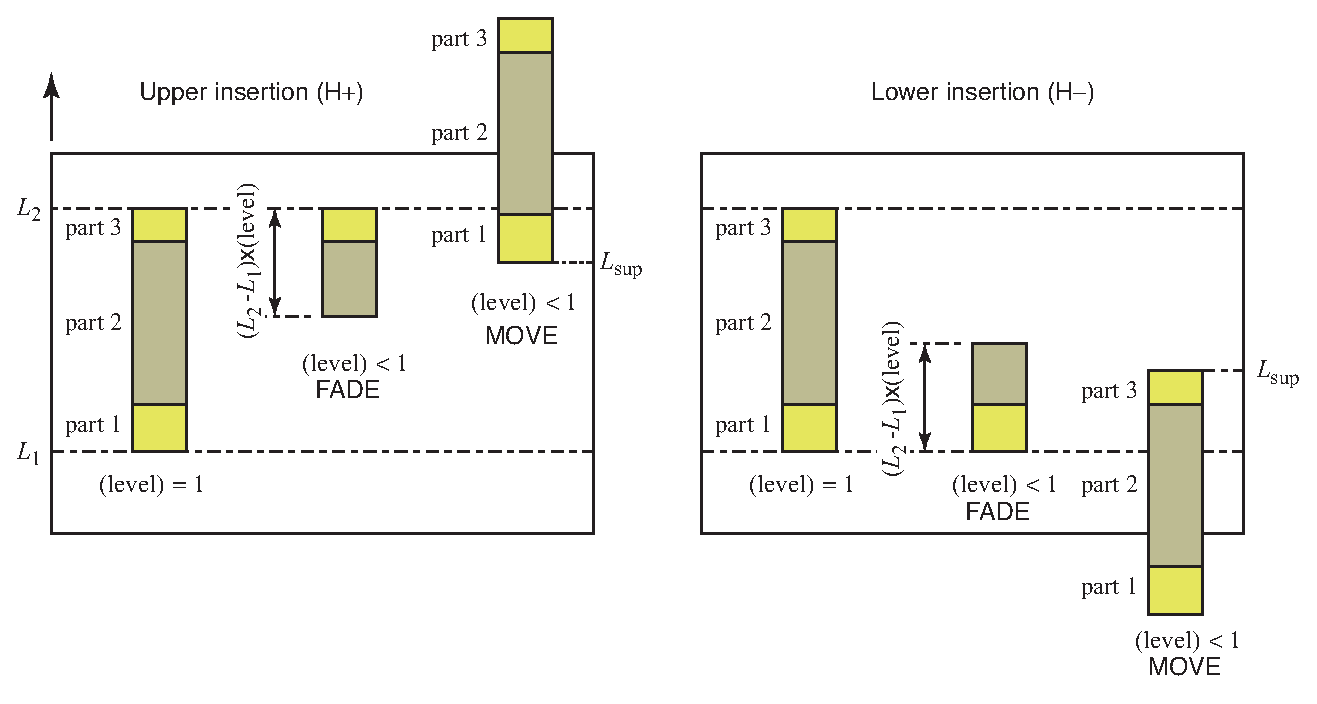
\includegraphics[scale=0.7]{Figures/rod.eps} 
\caption{Presentation of fully- and partially-inserted 3-part control rods.}\label{fig:rod}
  \end{center}
\end{figure}

\begin{DataStructure}{Structure \dstr{descdev}}
$[$ \moc{EDIT} \dusa{iprint} $]$\\
\moc{NUM-ROD} \dusa{nrod} $[~\{$ \moc{FADE} $|$ \moc{MOVE} $\}~]$ \\
( \dstr{dev-rod},  i = 1, \dusa{nrod} ) \\
$[$ \moc{CREATE}  \moc{ROD-GR} \dusa{ngrp}  ( \dstr{rod-group},  i = 1, \dusa{ngrp} ) $]$ \\
;
\end{DataStructure}

\noindent where
\begin{ListeDeDescription}{mmmmmmmm}

\item[\moc{EDIT}] keyword used to set \dusa{iprint}.

\item[\dusa{iprint}] integer index used to control the printing on screen:
= 0 for no print; = 1 for minimum printing (default value); larger values
produce increasing amounts of output.

\item[\moc{NUM-ROD}] keyword used to specify \dusa{nrod}.

\item[\dusa{nrod}] integer total number of the reactor rod-type devices.
This number must be greater than 0.

\item[\moc{FADE}] fading rod keyword. A fraction of the fully inserted rod vanishes (default option).

\item[\moc{MOVE}] moving rod keyword. The complete rod is moving (DONJON3-type movement).

\item[\moc{CREATE}] keyword used to create the rod-groups of devices.
The creation of groups is optional.

\item[\moc{ROD-GR}] keyword used to set \dusa{ngrp}.

\item[\dusa{ngrp}] integer total number of the rod groups to be created.
This number must be greater than 0.

\item[\dstr{dev-rod}] structure describing the input data for each individual rod.
 
\item[\dstr{rod-group}] structure describing the input data for each group of rods.

\end{ListeDeDescription}

\vskip 0.2cm

\subsubsection{Description of dev-rod input structure}\label{sect:devrodstr}

A rod position is referred by its \dusa{3-D} Cartesian coordinates only.
Note that the devices positions can not overlap. The input order of data
must be respected.

\begin{DataStructure}{Structure \dstr{dev-rod}}

\moc{ROD} \dusa{id} \\
~~\moc{ROD-NAME} \dusa{NAME} \\
~~\moc{AXIS} $\{$ \moc{X} $|$ \moc{Y} $|$ \moc{Z} $\}$ \\
~~\moc{FROM} $\{$ \moc{H+} $|$ \moc{H-} $\}$  \\
~~$[$ \moc{LEVEL} \dusa{value} $]$ \\
~~$[$ \moc{SPEED} \dusa{speed} $]$ \\
~~$[$ \moc{TIME} \dusa{time} $]$ \\
~~$[[$ \moc{MAXPOS}  (\dusa{pos}(i), i = 1, 6) \moc{DMIX} \dusa{mix1} \dusa{mix2} $]]$ \\
\moc{ENDROD}
\end{DataStructure}

\noindent where
\begin{ListeDeDescription}{mmmmmmmm}

\item[\moc{ROD}] keyword used to specify the rod \dusa{id} number.

\item[\dusa{id}] integer identification number of the current rod. Each
rod-type device must be assigned a unique \dusa{id} number, given in
an ascending order ranging from 1 to \dusa{nrod}.

\item[\moc{ROD-NAME}] keyword used to specify the rod \dusa{NAME}.

\item[\dusa{NAME}] \texttt{character*12} name of the current rod. In general,
this name is composed by the rod specific type (e.g. SOR, ZCR, etc.) followed
by its sequential number (e.g. 01, 02, etc.).

\item[\moc{AXIS}] keyword used to specify the rod movement axis.
A rod can be displaced along only one of the axis.

\item[\moc{X}] keyword used to specify that a rod is displaced along X axis.

\item[\moc{Y}] keyword used to specify that a rod is displaced along Y axis.

\item[\moc{Z}] keyword used to specify that a rod is displaced along Z axis.

\item[\moc{FROM}] keyword used to specify the insertion side of geometry.
The rod-devices can be inserted into the reactor core from only one side of
geometry. For example, some vertically moving devices can be inserted only
from the top, whereas other only from the bottom.

\item[\moc{H+}] keyword used to specify that a rod will be inserted into
reactor core from the highest position (e.g. from the top for vertically moving
rod-device).

\item[\moc{H-}] keyword used to specify that a rod will be inserted into
reactor core from the lowest position (e.g. from the bottom for vertically
moving rod-device).

\item[\moc{LEVEL}] keyword used to specify the actual rod insertion
level \dusa{value}. By default, the rod insertion level is left undefined.

\item[\dusa{value}] real positive value of the rod insertion level. This
value is used to compute the actual rod position in the reactor core.
The rod insertion level is minimal (\dusa{value} = 0.0) when the rod is
completely withdrawn, and it is maximal (\dusa{value} = 1.0) when the
rod is fully inserted. For the partially inserted rod the insertion level
must be: 0.0 $<$ \dusa{value} $<$ 1.0

\item[\moc{SPEED}] keyword used to specify \dusa{speed}. By default, the speed is left undefined.

\item[\dusa{speed}] real positive value of the rod movement speed,
given in cm/s. This value is needed only for the reactor regulating purpose.

\item[\moc{TIME}] keyword used to specify \dusa{time}. By default, the insertion time is left undefined.

\item[\dusa{time}] real value of time for the rod insertion (or extraction),
given in sec. This value is needed only for the reactor regulating purpose.

\item[\moc{MAXPOS}] keyword used to specify the full-inserted
coordinates of a rod part. The sequence of \moc{MAXPOS} and \moc{DMIX} data structures is
repeated for each part making the rod.

\item[\dusa{pos}] real array containing 3-D Cartesian coordinates of the
full-inserted rod. This is the limiting rod position in the reactor core, which
may or may not be the same as the actual rod position. These coordinates
must be given in the order: X$-$, X$+$, Y$-$, Y$+$, Z$-$, and Z$+$.

\item[\moc{DMIX}] keyword used to specify \dusa{mix1} and \dusa{mix2}.

\item[\dusa{mix1}] first of two integer rod mixture indices. Index \dusa{mix1} corresponds to the perturbed
cross sections.

\item[\dusa{mix2}] second of two integer rod mixture indices. Index \dusa{mix2} corresponds to the reference
cross sections. Indices \dusa{mix1} and \dusa{mix2} will be used to compute
the incremental cross sections in the \moc{NEWMAC:} module.

\item[\moc{ENDROD}] keyword used to end the rod description.

\end{ListeDeDescription}

\subsubsection{Description of rod-group input structure}\label{sect:rodgroupstr}

The partition of devices into groups is very useful when the same action is
to be applied to several rods, e.g. setting of new parameters (using the
\moc{DSET:} module) or rods moving (using the \moc{MOVDEV:} module).

\begin{DataStructure}{Structure \dstr{rod-group}}

\moc{GROUP-ID} \dusa{igrp} $\{$ \moc{ROD-ID}
$[[$ \dusa{id} $]]$  $|$  \moc{ALL} $\}$ \\

\end{DataStructure}

\noindent where
\begin{ListeDeDescription}{mmmmmmmm}

\item[\moc{GROUP-ID}] keyword used to set \dusa{igrp} number.

\item[\dusa{igrp}] integer identification number of a group to be created.
Each rods group must be assigned a unique identification number, given
in ascending order ranging from 1 to \dusa{ngrp}.

\item[\moc{ROD-ID}] keyword used to set the rod \dusa{id} numbers.

\item[\dusa{id}] integer identification numbers of rods which belong
to the same group \dusa{igrp}. A particular rod (or several rods) may
belong to different groups, but it could not be repeated inside the same
group. The total number of rods in any group must be between
1 and \dusa{nrod}.

\item[\moc{ALL}] keyword used to specify that all rods
will belong to the same group \dusa{igrp}.

\end{ListeDeDescription}
\clearpage
